\documentclass[conference]{IEEEtran}

\usepackage{cite}
\usepackage{amsmath}
\usepackage{graphicx}
\usepackage{fancyvrb}

\begin{document}

\title{Odd Ball Weighing Problems}

\author{\IEEEauthorblockN{Andrew~Mihal}
\IEEEauthorblockA{Hobbyist\\
Email: andrewcmihal@gmail.com}
}

\maketitle

\begin{abstract}
A classic problem in recreational mathematics is to identify an incorrectly-weighted ball in a set of $N$ otherwise identical balls.
The challenge is to use a balance scale a maximum of $W$ times, where $W$ is typically much smaller than $N$.
The solution must identify which ball has the incorrect weight and whether the ball is heavier or lighter that the rest.
We propose a collection of SAT benchmarks that solve this problem for various configurations.
\end{abstract}

\section{Problem Description}

This brainteaser has appeared in the literature in numerous variations for many years.
It is sometimes called the Odd Coin Problem or the Counterfeit Coin Problem.
The specific variation addressed in this paper is described by Bundy~\cite{b2}.
Students are usually tasked with solving the problem first with 9 balls and 3 weighings,
and then are challenged with the more complicated 12 ball, 3 weighing version.
It is clear that the ternary nature of the weighing outcomes is critical to the solution.

We implement a SAT-based solution to this puzzle that generalizes to an arbitrary number of balls $N$ and number of weighings $W$.
Combined with various symmetry-breaking strategies, these puzzles create instances that are useful for benchmarking
the performance of SAT solvers.

Constructive solutions to this puzzle are known, for example the solution due to Wert~\cite{b3}.
In this work we make the simplifying assumption that the balls to be weighed are determined \emph{a priori}. That is,
the choice of what to weigh next is not dependent on the outcome of the previous weighings.
Wert's solution in comparison has decision branches.

Some variations provide a known-good ball, or provide known counterweights, or give away the information that the odd ball
is lighter or heavier, or provide the specific delta weight between the good balls and the odd ball.
We do not address these variations.
We assume that the odd ball weight varies by only $\epsilon$ and therefore the same number of balls must be on both sides of the scale
for every weighing.

Our solution determines the set of balls on the left and right sides of the scale for each of the $W$ weighings.
The outcomes of the weighings are then looked up in a truth table that tells which ball is wrong and whether it is light or heavy.

\begin{figure}[!t]
\centerline{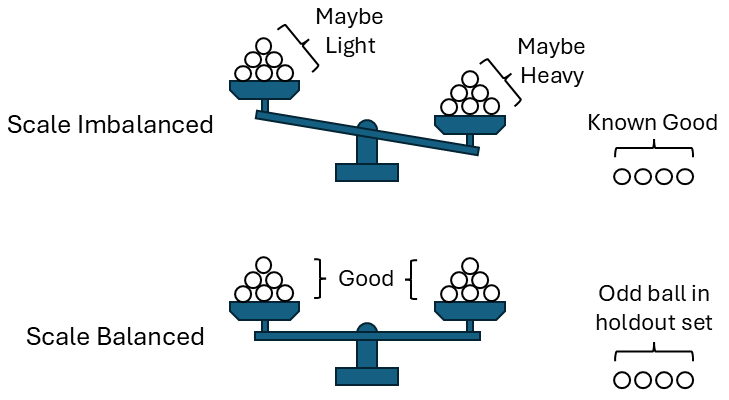
\includegraphics[width=\linewidth]{scale.png}}
\caption{Weighing Result Implications}
\label{scale}
\end{figure}

\section{SAT Encoding}

The Oddball program, available on GitHub~\cite{b1}, is implemented in Python using Z3Py.
The formulation uses an $W \times N \times N$ array of Boolean variables $B$,
where $B[w, n_1, n_2]$ indicates that ball $n_1$ is on the left side of the scale and ball $n_2$ is on the right side of the scale
in weighing $w$.
At\nobreakdash-Most\nobreakdash-1 cardinality constraints are applied to ensure that a ball does not appear on both sides of the scale
at the same time, or appear more than once on the same side of the scale.

A second set of Boolean variables $T$ model the truth table.
Variable $T[r, b, e]$ indicates that row $r \in [0, 3^W)$ has the outcome that ball $b \in [0, N)$ has error $e \in [-, +]$,
meaning that ball $b$ is light or heavy respectively.
Each truth table row must imply at most one ball-error combination.
Every ball-error combination must appear at least once in the truth table.

The outcome of each weighing implies possibilities about the location and error of the odd ball (see Figure~\ref{scale}).
If the scale is balanced, we know that all of the balls on the scale are good and the odd ball must be in the holdout set
that is not on the scale.
If the scale is imbalanced, we know that the odd ball must be on the scale.
It could be a light ball on the light side of the scale, or it could be a heavy ball on the heavy side of the scale.
All the balls in the holdout group are known to be good.

For each truth table row $r$, the outcomes of the $W$ weighings are known, and implications can be added to the formula
between the $B$ variables and the $T$ variables for that row.

The goal of the SAT solver is to choose pairs of balls to weigh in each weighing such that each truth table row implies
at most one result and all possible results appear at least once in the truth table.

The Python program can solve the formulation directly with Z3, or it can export CNF or SMT2 formats.
It can also re-import certificates to print and verify solutions generated by an external solver.

\section{Example Solution}

The following example solution is for the $N=12, W=3$ configuration.
The first section shows the sets of balls to place on the scale for each weighing.
The second section gives the truth table that maps the weighing outcomes to ball-error results.
The weighing outcome $<$ indicates that the left side of the scale is lighter than the right,
$=$ means the scale is balanced, and $>$ means the left side is heavy.

\begin{small}
\begin{BVerbatim}

Solution:
W0: [ 1,  2,  3,  6] <=> [ 0,  4,  5,  7]
W1: [ 1,  2,  7,  9] <=> [ 0,  6,  8, 10]
W2: [ 3,  5,  6, 10] <=> [ 0,  2,  8, 11]

Truth Table:
ix  W0  W1  W2   Result
 0   <   <   <   0+
 1   <   <   =   1-
 2   <   <   >   2-
 3   <   =   <   3-
 4   <   =   =   4+
 5   <   =   >   5+
 6   <   >   <   6-
 7   <   >   =   7+
 8   <   >   >
 9   =   <   <   8+
10   =   <   =   9-
11   =   <   >   10+
12   =   =   <   11+
13   =   =   =
14   =   =   >   11-
15   =   >   <   10-
16   =   >   =   9+
17   =   >   >   8-
18   >   <   <
19   >   <   =   7-
20   >   <   >   6+
21   >   =   <   5-
22   >   =   =   4-
23   >   =   >   3+
24   >   >   <   2+
25   >   >   =   1+
26   >   >   >   0-
\end{BVerbatim}
\end{small}

\section{Symmetries}

The problem has a few symmetries that can be exploited for better solver performance.

First, the problem is symmetric under permutations of the ball labels.
This symmetry can be broken with an ordering constraint on the ball numbers as they appear in the truth table.
Each row can imply no result (since the number of ball-error combinations may be less than $3^W$),
or the opposite error for a ball that has already appeared in the truth table, or it can imply an error
for the sequentially next ball that has not yet appeared.
This symmetry-breaking strategy was used for the example solution above.

An alternative that weakly breaks the label permutation symmetry is to enforce an ordering on the balls
that are placed on the scale in the first weighing. Pair 0,1 must be placed on the left and right sides first,
followed by pair 2,3, pair 3,4 and so forth.
The solver is free to choose how many pairs to weigh in the first weighing but they must appear in this order.
This strategy is weaker than the first because it still permits label permutations of the balls in the first holdout set.
Nevertheless this is an option provided by the program to improve the variety of generated instances.

Second, the truth table itself has mirror symmetry top-to-bottom.
This is a consequence of symmetry around the odd ball's error.
Imagine that the odd ball is on the scale and the scale is therefore imbalanced.
If the error on the ball is flipped, then the scale will also flip.
In any truth table row, if all the $<$ and $>$ outcomes are reversed, then the result must be the same ball number but with the opposite error.

Note that the middle row of the truth table with all $=$ outcomes cannot imply a result.
We know that the odd ball must be in the holdout set for every weighing.
This can be enough information to uniquely determine the odd ball, but not whether it is lighter or heavier than the others.

The truth table mirror symmetry can be exploited by only solving for the top half of the truth table in the SAT formulation.

\section{Benchmarks}

Configurations with $N \approx 50$ and $W=5$ can be solved by Kissat~\cite{k1} in the 10 to 20 minute range.
For our proposed benchmarks we generate examples around this point as well as some in the $N \approx 10$, $W=6$ range.
All are SAT.

For UNSAT instances, we could generate examples with $N > (3^W - 3) / 2$ (the maximum solvable $N$ for any $W$).
The $N=13$, $W=3$ instance is trivial for Kissat and the $N=40$, $W=4$ instance takes more than one hour, so they are not suitable
benchmarks.
Instead, we use an intentionally broken version of the truth table mirror symmetry strategy to generate UNSAT instances that take
Kissat up to 45 minutes to solve.
The broken strategy forces the balls to appear sequentially in the top half of the truth table without any empty rows.

\section{Conclusion}

This work was motivated while the author was helping math students with their homework during ski week in Austria.
The $N=12$, $W=3$ problem was given as a bonus challenge with the implication that it might not be solvable.
One student asked ChatGPT to solve the problem and ChatGPT said it was impossible.
The student, predisposed to stopping work anyway, decided to believe the AI and gave up.
This made the author upset.

While the approach used in this paper may not be optimal, it has been able to solve problems up to $N=36$, $W=6$
with 15 minutes of Kissat runtime.

\begin{thebibliography}{0}
\bibitem{b1} A. Mihal. ``Oddball,'' 2025, GitHub repository. [Online]. Available: https://github.com/acmihal/oddball
\bibitem{b2} B. Bundy. ``The Oddball Problem,'' 1996/7, Mathematical Spectrum, v 29, no 1, pg 14--15
\bibitem{b3} J. Wert. ``Odd Coin Problems,'' [Online]. Available: https://cut-the-knot.org/blue/OddCoinProblems.shtml
\bibitem{z3} L. De Moura and N. Bj{\o}rner. ``Z3: An Efficient SMT Solver,'' In TACAS'08. 337--340
\bibitem{k1} A. Biere et al. ``CaDiCaL, Gimsatul, IsaSAT and Kissat Entering the SAT Competition 2024''. In Proc. SAT Comp. 2024. 8--10
\end{thebibliography}

\end{document}
